\documentclass[11pt]{report}

\usepackage{subfig}
\usepackage[a4paper, top=1in, bottom=1in, left=1in, right=1in,, headheight=1in, headsep=5pt]{geometry} 
\usepackage[english]{babel} 
\usepackage{graphicx} 
\usepackage{fancyhdr}
\usepackage{float}
\usepackage{acronym} 

%\usepackage{natbib}
%\usepackage[backend=biber,style=alphabetic,sorting=ynt]{biblatex}
%\bibliographystyle{plain}
%\bibliography{bib/bibliography.bib} %Import the bibliography file


%\renewcommand{\headrulewidth}{0pt} % Remove header line
\renewcommand{\footrulewidth}{0.1pt} % Remove header line
% Redefine \chaptermark to avoid chapter title in \leftmark
\renewcommand{\baselinestretch}{1.05}



\pagestyle{fancy} % Enable custom headers/footers
\fancyhf{} % Clear default header/footer

\fancyfoot[C]{A project on the master’s in industrial Electronics and Computers
Engineering by the professors Luis Gonçalves and Sérgio Lopes 2024/2025}
\fancyfoot[R]{\newline\newline\thepage}

%\fancyhead{}
\fancyhead[R]{\footnotesize\nouppercase{\leftmark}}
\fancyhead[LO]{\footnotesize\nouppercase{\leftmark}}
\fancyhead[R]
{


\includegraphics[width=0.17\textwidth]{images/logos/TOP_ENG_LOGO.png}  % Adjust the width as necessary
%\caption{This is a Header_image}
\label{fig:UM_LOGO}
\hspace{0.1cm}

\includegraphics[width=0.09\textwidth]{images/logos/TOP_CMEMS_LOGO.png}  % Adjust the width as necessary
%\caption{This is a Header_image}
\label{fig:CMEMS_LOGO}

}



\begin{document}
    \begin{titlepage}
        \centering
\begin{figure}[h!]  % The 'h!' position option forces the image to be placed here
    \centering
    
\includegraphics[width=0.3\textwidth]{images/logos/ENG-EN.png}  % Adjust the width as necessary
    %\caption{This is a sample image}
    \label{fig:UM logo}
    \hspace{0.1cm}
    
\includegraphics[width=0.6\textwidth]{images/logos/CMEMS.png}  % Adjust the width as necessary
    %\caption{This is a sample image}
    \label{fig:CMEMS logo}
    

\end{figure}
\vspace{0.25in}
\large
Master’s in Industrial Electronics and Computers Engineering \\
\vspace{0.15in}
\LARGE
University of Minho\\
\vspace{0.35in}
%\huge
\hrule

\vspace{0.2in}
\textbf{\Huge 5S \\ \Large Sensoring System for Surface Sea Streams}
\vspace{0.2in}

\hrule
\vspace{0.2in}
\large
Integrative Project in Industrial Electronics and Computers
\vspace{4in}

\textbf{Author:}
Vinicius Carvalho PG56208

\vspace{0.1in}

\textbf{Professors:}
Luis Gonçalves and
Sérgio Lopes

\vfill

2024/2025
    \end{titlepage}
    \pagenumbering{roman}
    %index table of images and acronims
    \tableofcontents  
    \listoffigures
    \listoftables
    \textbf{\Huge Acronyms} %remove indentation
    \normalsize
    \begin{acronym}[UART] % Give the longest label here so that the list is nicely aligned
        \acro{UART}{Universal asynchronous receiver/transmitter}
        \acro{LTE}{Long-Term Evolution}
        \acro{ADC}{Analog to Digital Converter}
        \acro{IMU}{Inertial Measurement Unit}
        \acro{PCB}{Printed Circuit Board}
        \acro{CMEMS}{Center for Microeletromachanical Systems}
        \acro{STM32}{}
        \acro{DMA}{Direct Access Memory}
        \acro{IoT}{Internet of Things}
        \acro{GPS}{}
        \acro{JSON}{}
        \acro{DB}{Data Base}

    \end{acronym}
    
    \newpage

    \pagenumbering{arabic}
    \setcounter{page}{1}

    \chapter{Project Plan}
    This chapter will briefly talk about the 5S Drifter project motivations as well their function as a product developed 
    by the Minho's University under supervision by the professors Luis Gonçalves and Sérgio Lopes.
\section{Introduction}
Under the course unity of Integrative Project in Industrial Electronics and Computers the students must
apply for professors projects in order to integrate unde their respective laboratories and start to undertand the pace
demanded on the Master's final paper.

This project, given by the professor Luis Gonçalves and Sergio Lopes under the CMEMS laboratory,
has the main porpouse to create a drifter for data aquisition. As a multi-themed project, this report will
explore multiple areas, as the PCB design for hardware and firmware manufacture, software design under the idea to optimize
the execution allowing for better performance. The main goal is to have the final product afloat at the end of the simester.

\subsection{Problem Statement}
The ocean is one of the man greatest mistery even before the written history. Humanity made the world ours over the water, 
from the Portuguese greatests discoveries, braving the raging ocean to the newst oil tanker demanding ever newer technology
in order to tame the sea for safer and smother sailing.

Nowadays cientists belive only 5\% of the ocean is discovered with the actual technology witch means that humanity 
know as much about our so grate sky as our own seas. 5S ocean drifter is a equipament made to acquire date from 
superficial sea streams and expand the oceangrapgh knowledge about it.

Better knowledge of the ocean lead to further development in diverse areas. Granting safety,
security and efficiency.

5S, an acronym for Sensoring System for Surface Sea Streams is a lowcost, lowpower solution to acquire
said data with the focus to last autonomously for the longest time possible. The drifter has to attain its GPS
coordenates in order to track its current and avarege velocity, alongside with the water temperature and a accelerometer 
information to gether information about the wave intencity. All this data will be transmitted by a protocol,
 yet to be defined, with a JASON format in order to be read by a database that allready is implemented.  


\subsubsection{Transport}
Sadly, it isn't uncommon to see transport accidents being reported, and even worse, for it to be a gigantic problem.
Some of these accidents are caused by poor mapping of sea conditions, tankers spilling oil, fishing vessels capsizing, leading
to financial problems and even loss of life. Even when there are no accidents, poor knowledge of tides results in higher energy consumption when routes are set against the currents.

A solution would be to create optimized shipping routes, minimizing accidents and improving energy efficiency while 
traversing the waves. Oil tankers could follow currents with lower fuel consumption. Fishing routes could become more
efficient, as their target species may swim with the tides based on temperature and speed. This would ease the workload,
making the activity less reactive and more predictable, aligning expected catch rates with reduced time and energy 
consumption.

A well-known example of a hazardous area is the Nazaré Canyon, where its unique shape creates enormous waves. 
Avoiding these waters is crucial for safer navigation.

\subsubsection{Ecology}


Habitats 

The placement of wave energy converters, a growing field under the energy generation, is one of the main problems the
technology faces. A good positioning improves the efficiency
\begin{center}
    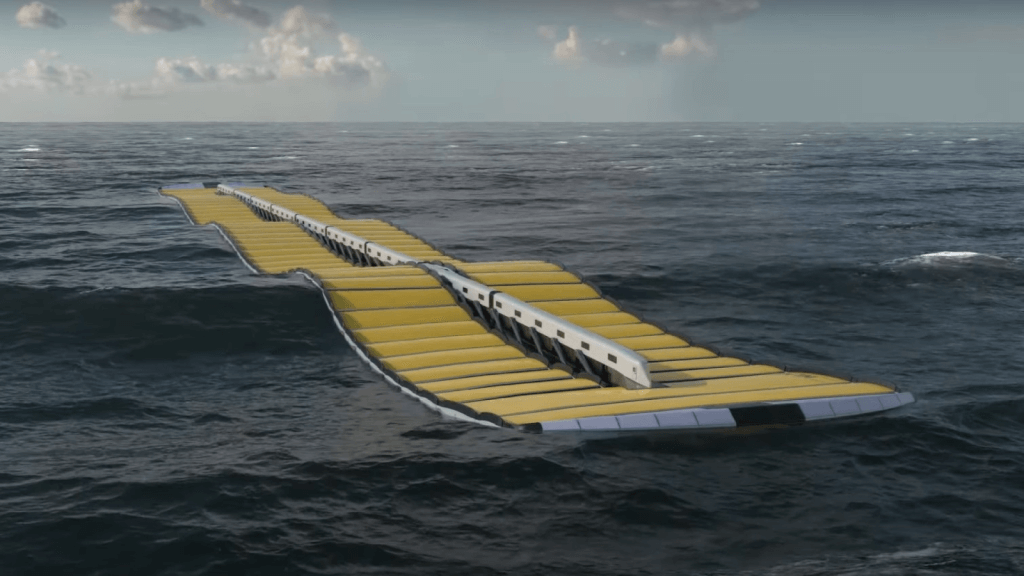
\includegraphics[width=0.7\textwidth]{images/chapter/introduction/renewable_energy.png}  % Adjust the width as necessary
    
    \label{fig:The Design of a Wave Energy Converter to Electricity}        
\end{center}

Renewable Energy 

\subsubsection{Oceanograpy}
Better undertanding of the Iberian Poleward Current (IPC)

\subsubsection{Geology}

Know where the sedimentation is leading to
\subsubsection{Sports}

\subsection{Problem Statement Analysis}

waterfall

vila do conde + ou - 10km mar adentro 2g 4g\\
mapa de alcance na costa\\
atenção ao clima \\
latencia / sampling / tamanho do cartão sd\\ 
autonomia de NO MINIMO 50 DIAS \\
consumo médio max 5mA \\
distancia da antena e da água \\
IMU caso tenha espaço para o consumo \\
SD memoria local \\
ADC a bateria \\
sensor de temperatura \\
database mongo db \\

    
    \newpage
    \chapter{Analysis}
In order to accomplish said objectives listed on the problem Statement Analysis, it is first
needed to enlist the embedded system components, this will help to choose a STM32 model as 
well the modules for this task without any over and under dimensions.

\begin{itemize}
    \item Microcontroller \\\hspace*{1cm} The STM32 CPU that will control the Embedded System.
    \item GNSS \\\hspace*{1cm} A module to acquire the world position in latitude and longitude.
    \item Mobile Communication \\\hspace*{1cm} The module with the ability to communicate wirelessly with MongoDB 
    \item Power Source \\\hspace*{1cm} The set of batteries the system will relay on for energy. It is stipulated that
    the system must have the autonomy of at least 30 days.
    \item SD Card Slot \\ Local long term memory in case of field transmission.
    \item Sensors:
    \begin{itemize}
        \item IMU \\\hspace*{1cm} System physical acceleration and angle data.
        \item Temperature Sensor \\\hspace*{1cm} Water Temperature data.
        \item Power Source Level Sensor \\\hspace*{1cm} Voltage reading data.
    \end{itemize}
\end{itemize}

As for the outer shell there are a few things to have in attention. 

\begin{itemize}
    \item The Antenna to floater distance, once the water interferes with the antenna signal.
    \item The float size, that needs to support all the weight and float, respecting the first topic.
    \item The drifter ballast, that will be the drifter core, located between the 
    floater and the temperature sensor tip. It should be heavy so the drifter points up, but it shouldn't exceed the 
    second topic demand 
    \item The Floater volume, as it has to balance the hole electronics and shell 
    weight.
\end{itemize}
This creates a first view of the system as a block diagram. Indicating the physical 
connection between each component. This won't define the 5S architecture, but it will serve
as an initial guide to build on.

\begin{figure}[H]
    \centering
    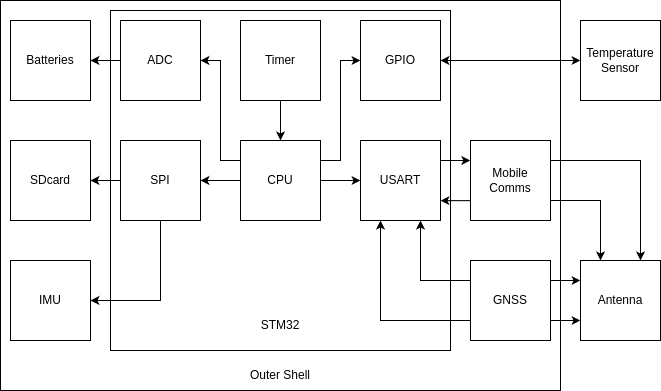
\includegraphics[width=0.9\textwidth]{images/diagrams/block_diagram/block_diagrams_3/blockdiagram_analysis.drawio.png}  % Adjust the width as necessary
    \caption{Block Diagram Initial Draft}
    \label{fig:Block Diagram Initial Draft}        
\end{figure}

The floater draft shows the initial concept of a drifter, as it has the above water 
antenna, a floater to counterbalance the buoy weight, and the temperature sensor. 
According to the blocked diagram.
%corrigir, falta a case no meio e ta mau recortado
\begin{figure}[H]
    \centering
    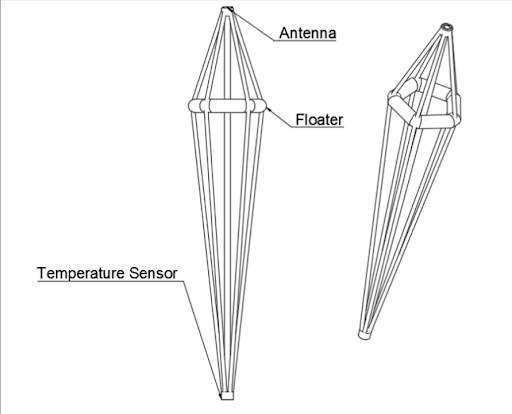
\includegraphics[width=0.7\textwidth]{images/diagrams/shell/unnamed.png}  % Adjust the width as necessary
    \caption{Floater Architecture Initial Draft}
    \label{fig:Floater Architecture Initial Draft}        
\end{figure}

\section{Requirements and Constraints}
\subsection{Requirements}
\begin{itemize}
    \item Search and selection of hardware components.
    \item Software design.
    \item PCB design.
    \item 5S outer shell 3D design.
    \item Actual product realization.
    \item Laboratory tests.
\end{itemize}
\subsection{Constraints}
\begin{itemize}
    \item Limited Team
    \item The project must be presented for evaluation within deadline.
    \item The project has to be validated at the ocean.
    \item The pretended autonomy has to be of a mouth at minimum.
\end{itemize}

%vila do conde + ou - 10km mar adentro 2g 4g\\
%mapa de alcance na costa\\
%atenção ao clima \\
\section{State of the art}
%%usar fotos do projeto no lab
Nowadays, there are a series of reasons in witch drifters are used. Usually, government 
departments, companies and universities with relations to oceanography, use drifter alike 
to research the local coast for the following reasons.

\begin{itemize}
    \item Border Control
    \item Climate Modeling
    \item Traffic management
    \item Aquaculture management
    \item Public oceanographic research
    \item Marine spatial planning
    \item Defense and security
\end{itemize}

5S drifter aims for \textbf{Climate Modeling}, \textbf{Public oceanographic} or even \textbf{Traffic management} research as this project main objective.
As the data for this project can be used, as stated in the \hyperref[sec:Problem Statement]{Introduction}, to model the environment
in order to better the quality of said topics.
\subsection{Copernicus Example}

The Copernicus Marine Service, component of Copernicus Programme of the 
European Union, has developed the SVP-BRST, a drifter for temperature and depth measurement.
Based on the SSP-B design, the updated version implements a HRSST in addition to the regular 
SST sensor, gathering the position with GNSS and transmitting the data using Iridium.
\begin{figure}[H]
    \centering
    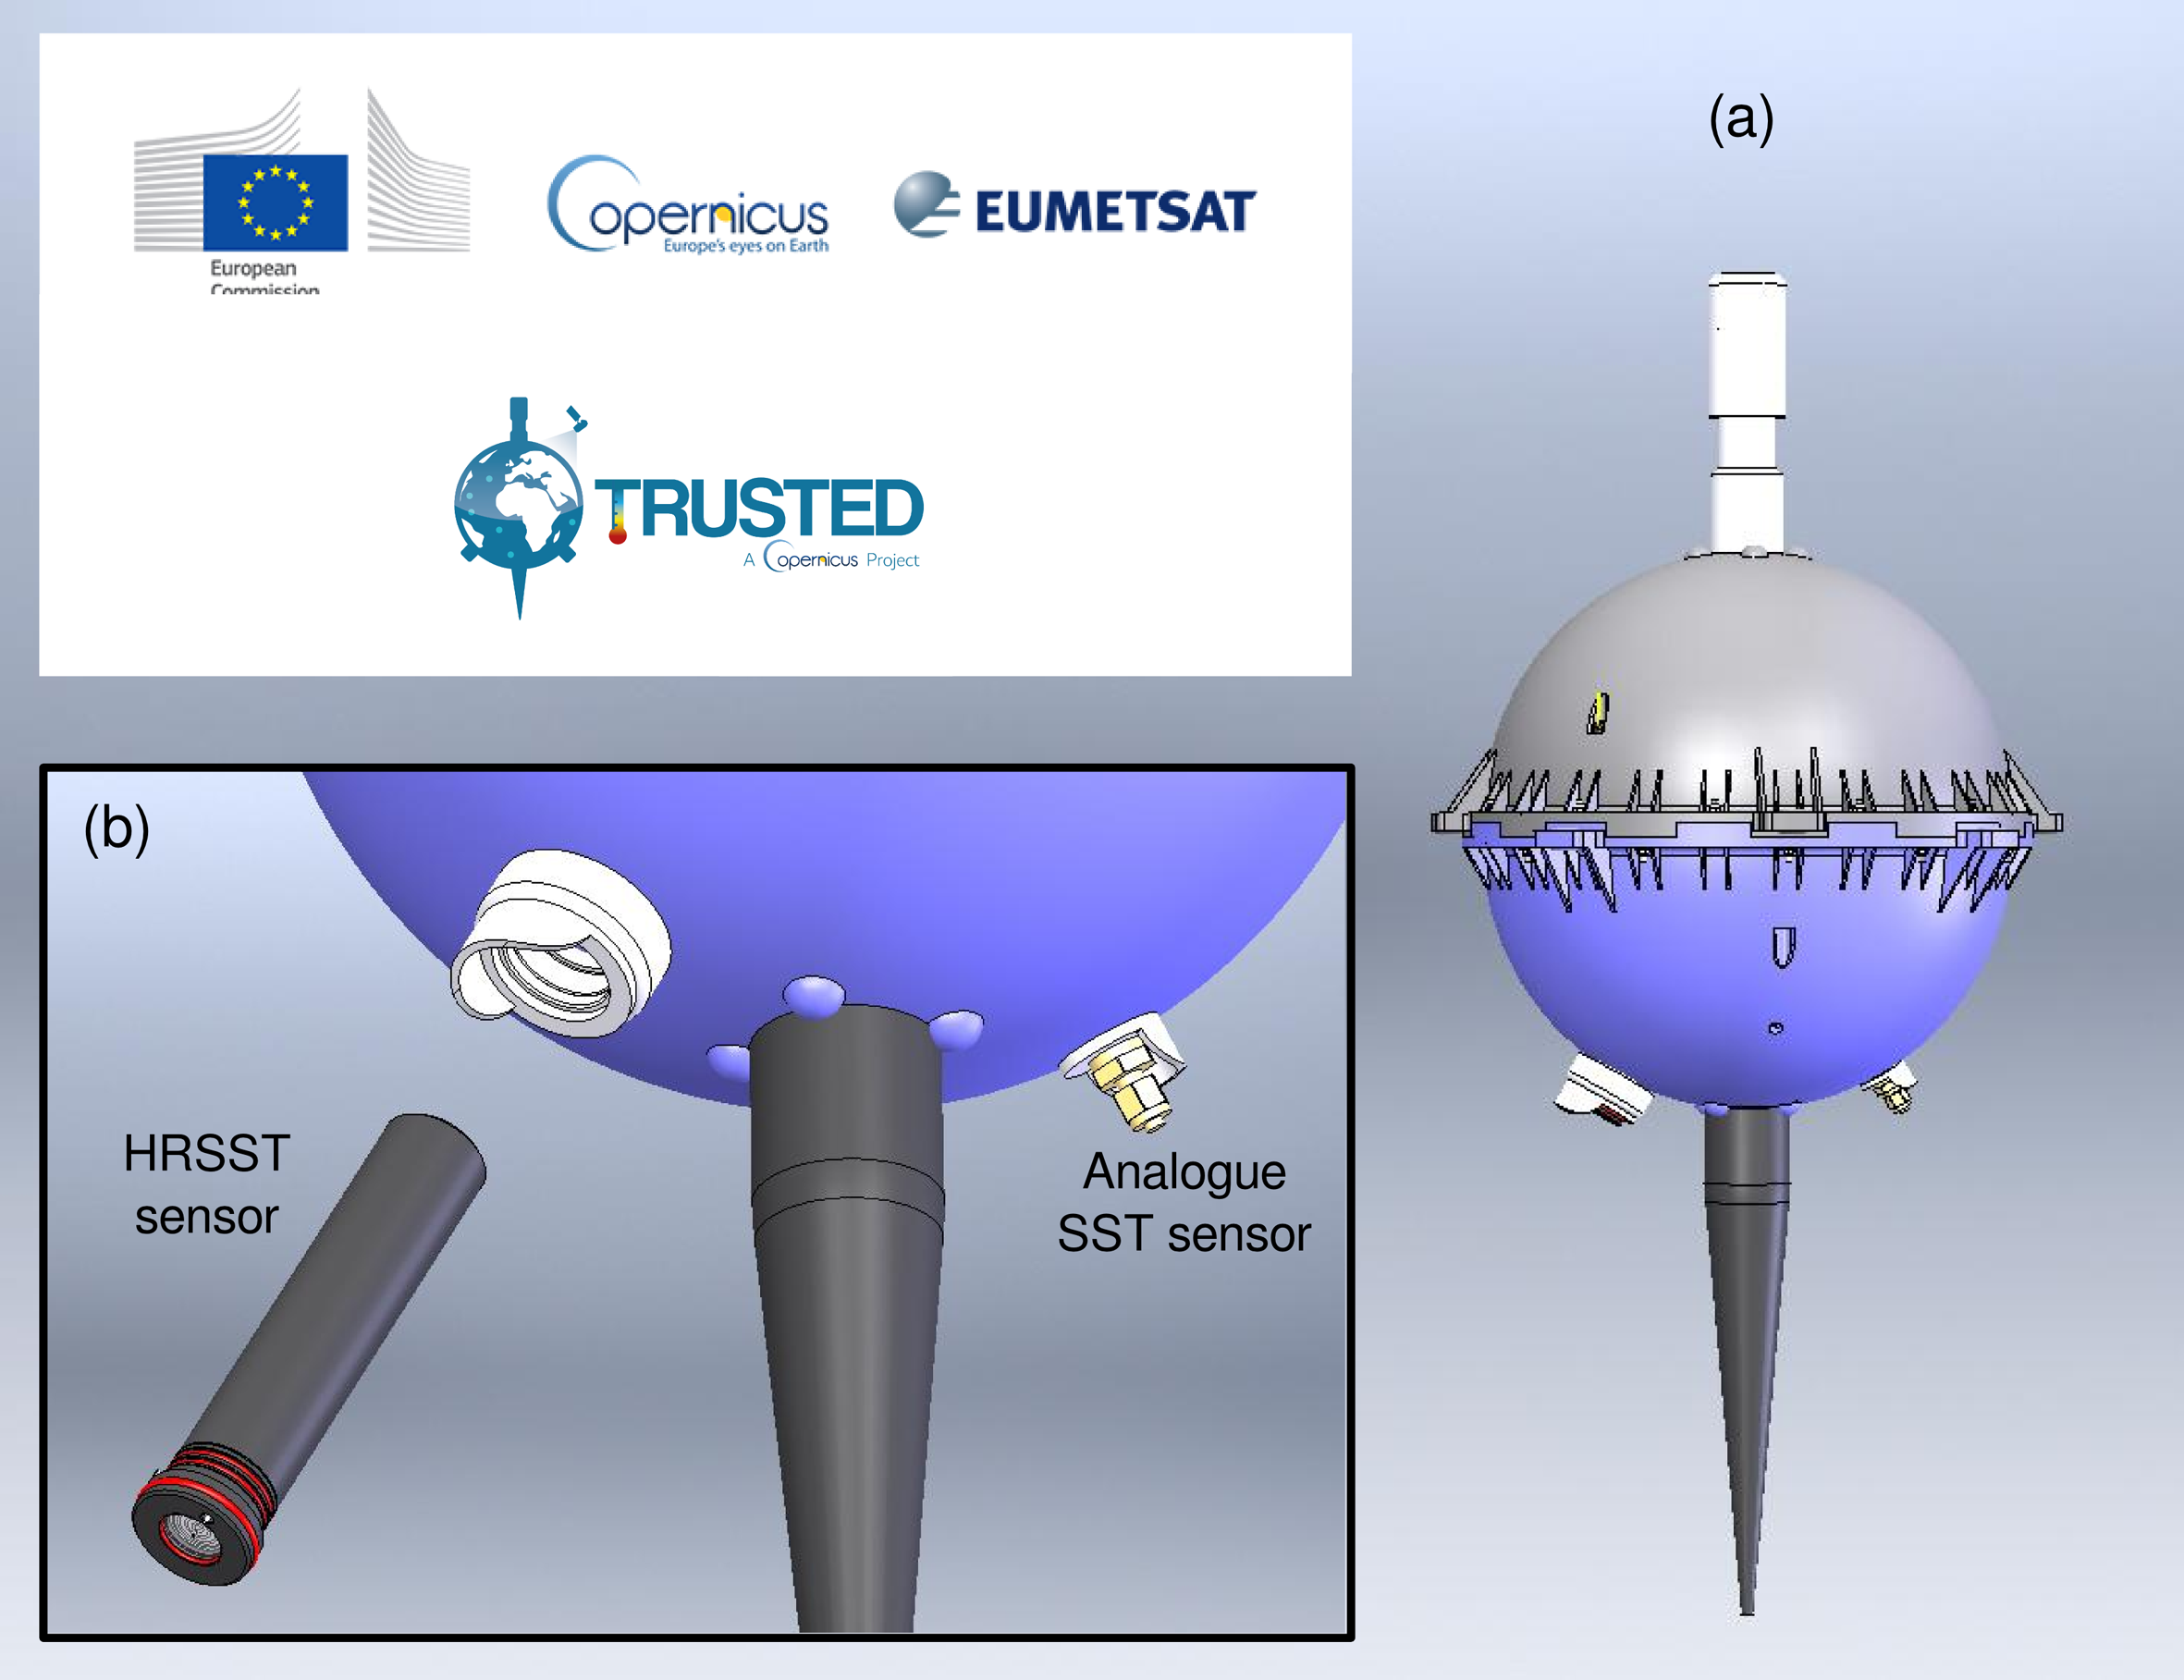
\includegraphics[width=0.55\textwidth]{images/chapter/analysis/svp.png}  % Adjust the width as necessary
    \caption{SVP-BRST Design}
    \label{fig:SVP-BRST Design}        
\end{figure}
The image shows the SVP-BRST model. The (a) image shows the hole model with the antenna the buoyant part ad the weight to point the buoy up.
As for the (b) image, shows the sensor's placement. 

\subsection{CMEMS Examples}
The CMEMS lab at the University of Minho combines expertise 
in microsystems engineering with environmental research to 
develop innovative ocean monitoring technologies. One of 
its key areas involves the design and deployment of autonomous 
drifters to collect real-time data on sea surface conditions 
and currents.

\subsubsection{SONDA}
The project proposes a complementary system for atmospheric
and oceanic monitoring using configurable probes launched by
high-altitude balloons. These probes can measure environmental
parameters from the stratosphere to the deep sea. After 
reaching the seafloor and collecting data (including acoustic 
imaging), the probe resurfaces and transmits the data via 
satellite. It then drifts until its material degrades. The 
system offers a low-cost, high-payload solution with 
limited positional accuracy.

%\begin{wrapfigure}{L}{0.4\textwidth}
%    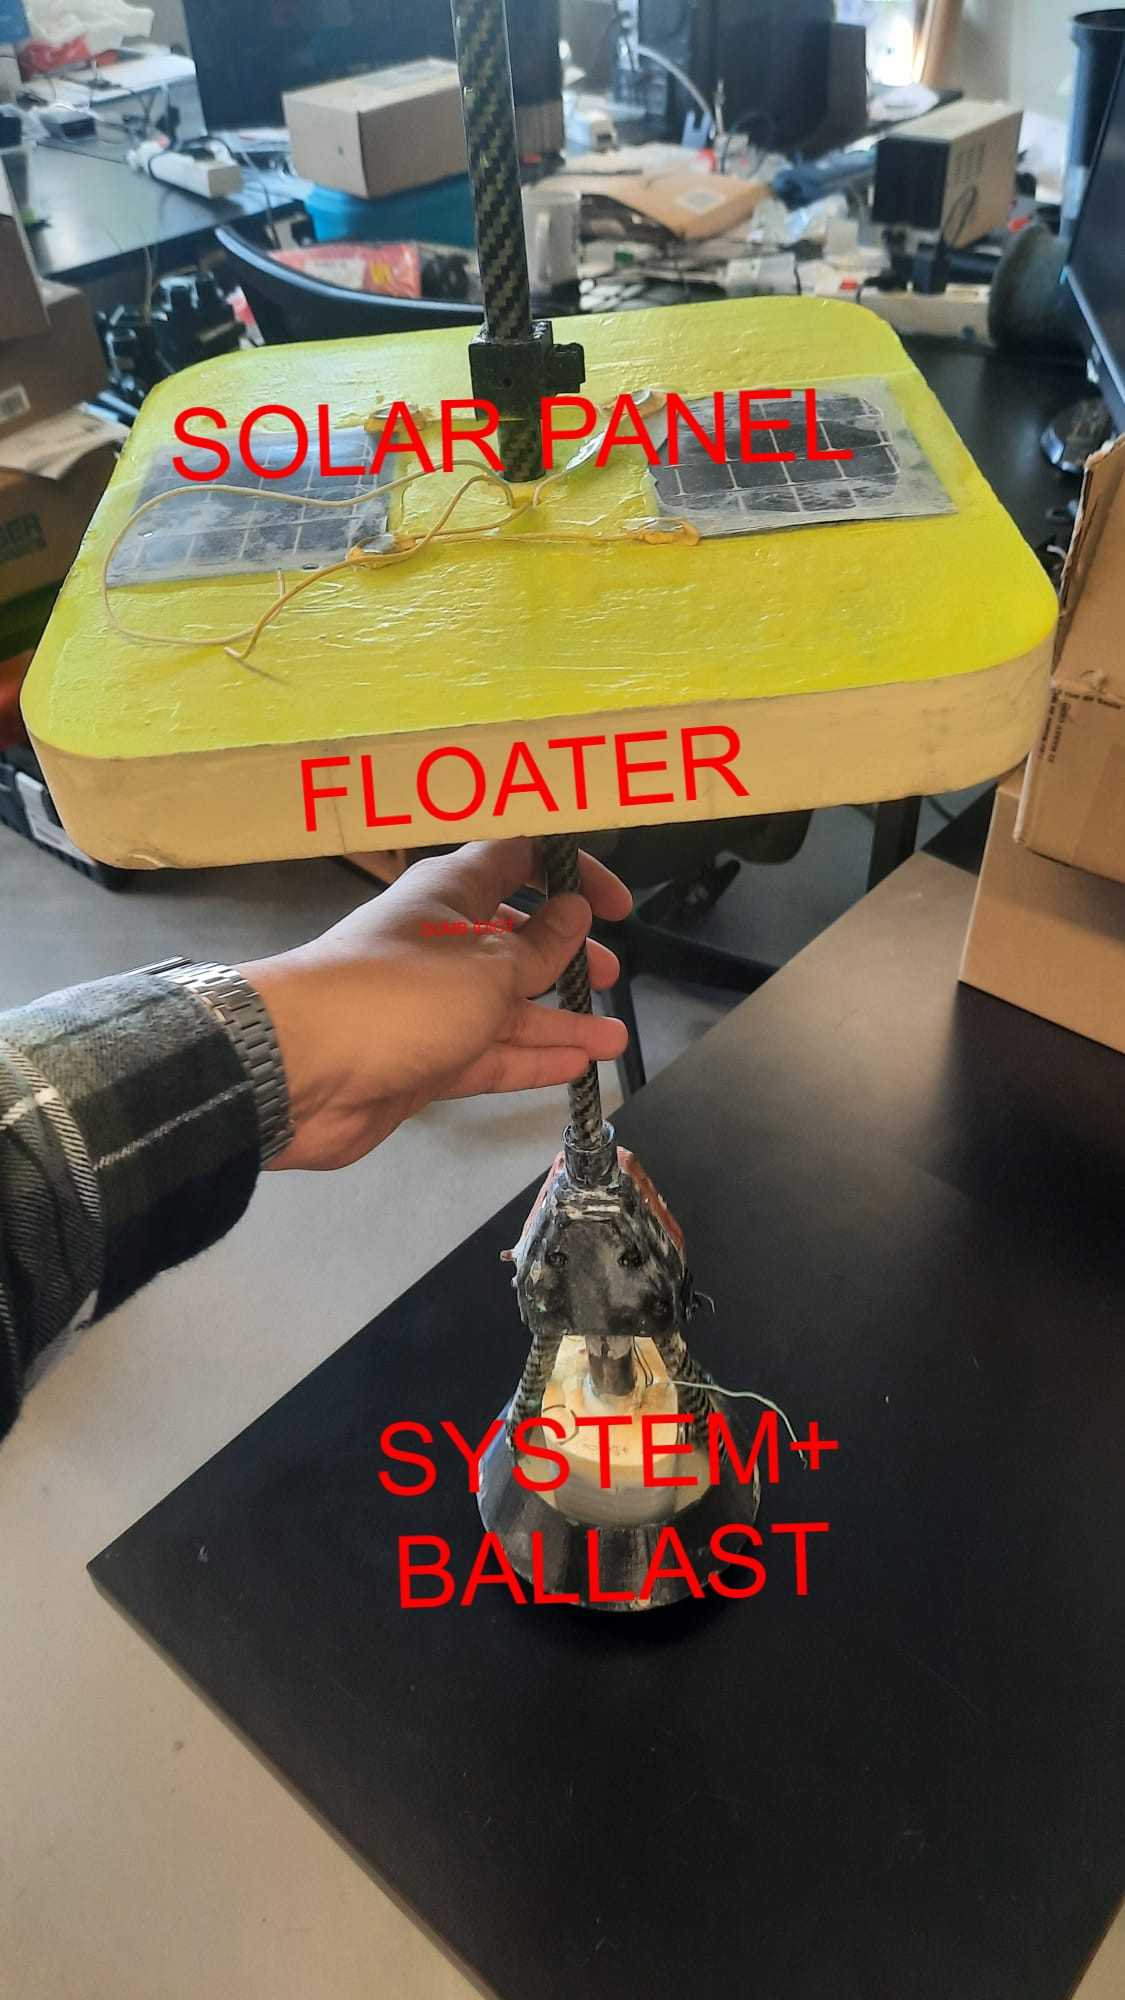
\includegraphics[width=0.25\textwidth]{images/chapter/analysis/sonda_edited.jpg}  % Adjust the width as necessary
%    \caption{SONDA drifter}
%\end{wrapfigure}

\subsubsection{NextSea}
A new approach of monitoring coastal and estuarine relevant variables is presented. MEMS
(Micro Electromechanical Systems), lab-on-chip and microelectronics are used to 
miniaturize and optimize main oceanic sampling. Beyond typical CTD (Conductivity, Temperature
and Depth), other oceanic variables are also monitored. The system also samples type of
phytoplankton and its concentration, pH, currents direction and intensity and turbidity.

\section{System Architecture}

Once studied what the system needs to follow, it is now needed to formulate a solution.
Here it will be used UML diagrams to convey the solution in question, whiteout real specifications
once this proposal works as a validation and organization to the problem as a formal language.

\subsubsection{Block Diagram}

As previously stated, a block diagram is a formal representation of the system components
and their connection. This one, shows how the peripherals communicate with the microcontroller STM32
as it considers connections with components outside the shell. Initially, as a first analysis
the communication protocol isn't yet defined. However, it will be used to narrow it down.

The diagram shows the SMT32 minimum peripherals: ADC, TIMER, GPIO, I2C / SPI, USART. However,
as it describes the hardware, it doesn't give a good notion on the system software. 

Some points to be considered are:
\begin{itemize}
    \item The temperature sensor communicate using the GPIO, as waterproof sensors, usually, use a driver with specific
    communication protocols.
    \item Mobile Comms is the protocol that will be used to send information to the database. Yet to be chosen. 
    \item GNSS and Mobile Comms for now communicate to the same Antenna, However it probably will use different antennas as different
    protocols require different frequencies to be used.
    \item The communication to the SDcard, uses SPI with STM32 below 64 pins. As it 
    doesn't include SDMMC supporting FatFS.
    \item The batteries power the hole system. Even if not shown.
    \item Depending on the implementation, the timer block will be the Sysclock, as 
    the RTOS may use by default.
\end{itemize}

\begin{figure}[H]
    \centering
    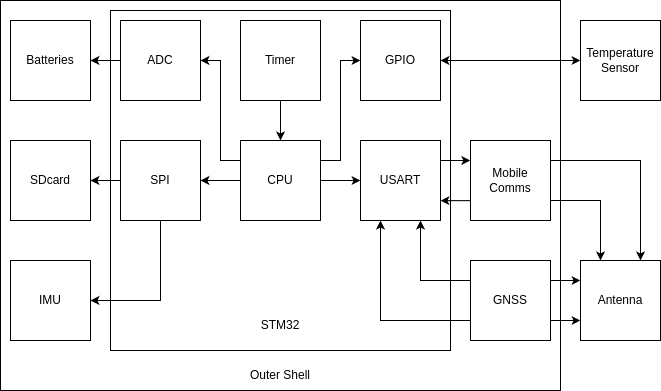
\includegraphics[width=0.9\textwidth]{images/diagrams/block_diagram/block_diagrams_3/blockdiagram_analysis.drawio.png}  % Adjust the width as necessary
    \caption{Block Diagram}
    \label{fig:Block Diagram}        
\end{figure}

\subsubsection{Use Case}

Now, for a software illustration, UML offers a user case, a diagram that exemplifies the system interactions and stimuli.

\begin{figure}[H]
    \centering
    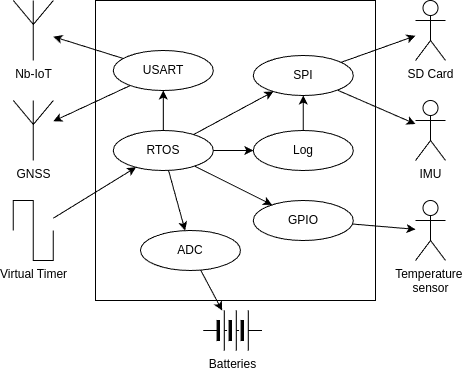
\includegraphics[width=0.6\textwidth]{images/diagrams/use_case/Use Case.drawio.png}  % Adjust the width as necessary
    \caption{Use Case Diagram}
    \label{fig:Use Case Diagram}        
\end{figure}

Now it is introduced to one main component that will be explored further, an RTOS. As it is stimulated by the timer, it will actvate the 
peripherals in a organized form, allowing a fast and efficient use of energy. Other component is the Log, a virtual memory that will store
temporary the information, only storing locally, once per cycle, reducing the SDcard entries.

\subsubsection{Sequence Diagram}

Once the software and hardware are planed, now a time related diagram will show the blocks interactions
as time passes.

First task sequence, a generic "Data Acquisition Task" shows the general behavior of a task focused to menage the sensors.

\begin{figure}[H]
    \centering
    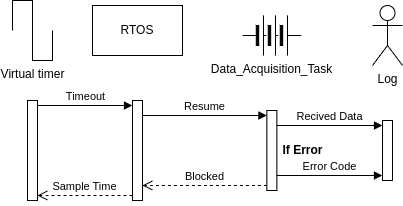
\includegraphics[width=0.7\textwidth]{images/diagrams/sequence_diagram/sequence_diagram_1/Sequence Diagram.drawio.png}  % Adjust the width as necessary
    \caption{Sequence Diagram of Sensor Task}
    \label{fig:Sequence Diagram of Sensor Task}
\end{figure}

Next, the second task sequence, there will be 2 tasks with the behavior to get the GNSS information, store it on log, then call for the Mobile Comms task to send the stored memory to the Database.
On the end, initiating the SDcard storage. 
\begin{figure}[H]
    \centering
    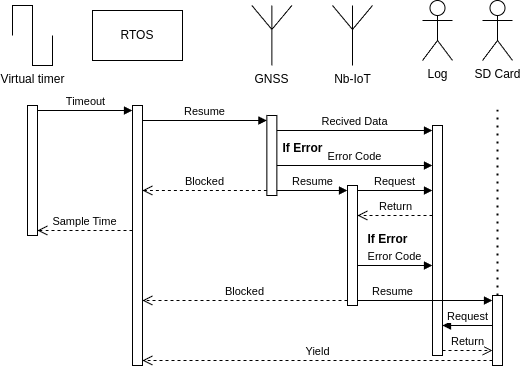
\includegraphics[width=0.7\textwidth]{images/diagrams/sequence_diagram/sequence_diagram_2/Sequence Diagram.drawio.png}  % Adjust the width as necessary
    \caption{Sequence Diagram for Sending and Archive Task}
    \label{fig:Sequence Diagram for Sending and Archive Task}        
\end{figure}

\subsubsection{Threads} 
Once this problem requires a list of tasks to be executed, using a OS will allow
a better project organization and performance with little to no impact in power consumption, 
even helping to menage the low power mode. However, the implementation will suffer, as the
codification as verification grows, so this topic may become an additional information 
by the end of the project.

As the ST uC offers a variety of RTOS, the implementation will be accessible with good support due to the
CMSIS v2 abstraction layer.

The division in Threads demands a separation in Priority levels, as the OS scheduler takes in consideration 
once both tasks are ready for execution.  

Setting a task priority it must take in vision the resources the task will use, the time it will take to execute said behavior
and the actual importance in matching it time constraints. In order to menage this level of complexity, the RTOS offers a set of
tools for tasks control that will be used for its synchronization and communication.
\begin{itemize}
    \item High Priority Threads \\ 
    Tasks that will handle the outer communication as GNSS and the internet integration will take the higher priority once, as will be handled
    by a peripheral, its execution will be faster, only using the USART interface for AC transmission. 
    \item Normal Priority Threads \\
    The only task here will be the one that has enough importance to be prioritized over the sensors but as the transmission begins it should release the processor
    for the outer communication.
    \item Low Priority Threads \\
    Tasks that only has to measure the sensors having no problem to be removed from the CPU execution
    once their execution is, in their majority, asynchronous.
    
\end{itemize}

%rescrever
\begin{figure}[H]
    \centering
    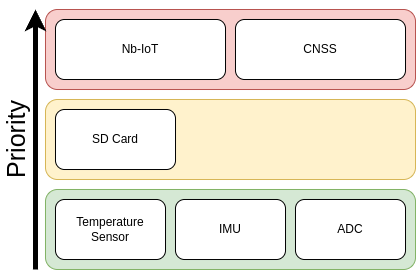
\includegraphics[width=0.7\textwidth]{images/diagrams/threads/thread.drawio.png}  % Adjust the width as necessary
    \caption{Thread Priority Stack}
    \label{fig:Thread Priority Stack}        
\end{figure}

Other important perspective, is to emulate the task behavior with the priorities in action. 
Showing a repetion of X times a group of data acquisition tasks, then ending with the second task sequence.
X yet to be defined as it first depends on the sample time. 
\begin{figure}[H]
    \centering
    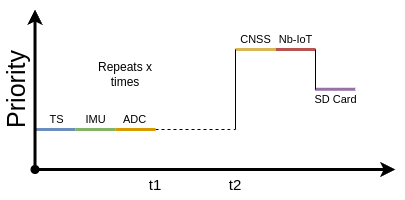
\includegraphics[width=0.7\textwidth]{images/diagrams/threads/graph/threads_graph.drawio.png}  % Adjust the width as necessary
    \caption{Thread Temporal Graph}
    \label{fig:Thread Temporal Graph}        
\end{figure}

Here up to t1 the system executes tasks, storing data, then entering low power mode until the next sample.
Then, at the end of the last repetition, at t2, stating the second task sequence. Then after the SDcard task behavior ends, as so do the cycle.
\subsubsection{Memory Abstraction (Log)} 

The final diagrams, are a exception to UML diagrams, As it only builds a data structure and a simple interface to interact with it.
Here the idea is to allow memory to be accessible while written by the system, optimizing the RTOS ITCs options.
\begin{figure}[H]
    \centering
    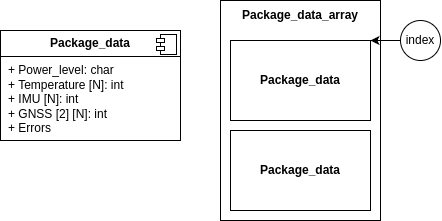
\includegraphics[width=0.7\textwidth]{images/diagrams/data_struct/package_data.drawio.png}  % Adjust the width as necessary
    \caption{Package data structure}
    \label{fig:Package data structure}        
\end{figure}


\begin{figure}[H]
    \centering
    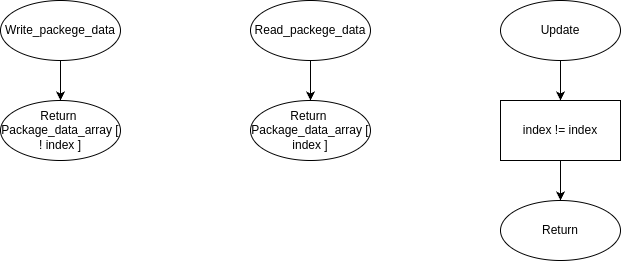
\includegraphics[width=0.75\textwidth]{images/diagrams/data_struct/fluxogram.png}  % Adjust the width as necessary
    \caption{Memory Flowchart}
    \label{fig:Memory Flowchart}        
\end{figure}


    \newpage
    \chapter{Design}
Now, once planed "What" is the system, it is needed to plan the "How" the system will be build in 
the implementation phase. Here is explained the components and the reason for it. As well
for the instructions on the system construction and realization.

\section{Analysis Review}

Taking in account the limited personal and time, some of what is specified in Analysis
has the scope reduced as to accomplish according to the requirements and constraints.
Using as inspiration the Copernicus SVP-BRST and the CMEMS labs previous experience,
the 5S can/ and will recall for used technology for easier design process.

The project then will be divided in three main parts; The Software, Hardware and the outer shell.
Then, lately, it will be shown the pieces of software used to accomplish this project. 

\section{Software}

As for software there will be two possible approaches for the problem, as the use of a RTOS
as stated on the Analysis, may require more time than it is worth. However, the use of a
RTOS, allow for a better control off timings and the Low Power mode. Either way, as the
implementation of both alternatives may differ, the overall design will remain the same. 

This section will first decide the protocol available, abstractions, then the possibility of using a RTOS

\subsection{Communication protocol}

The selection of a network protocol is a complicated process as it interests with several
factors that imply directly on the data to be acquired. To list the ones with more influence.

\begin{itemize}
    \item Distance
    \item Bit-Rate
    \item Signal Availability (SIM card and protocol local integration)
    \item Price per package
    \item Integrated GNSS Hardware
    \item Low Power
\end{itemize}

There are several protocols to choose from, so first it is needed to categorize the 
system needs and filter the list.

The first filter will be the distance. The IPC extends for kilometers along the shore, 
however signal along the shore can be mostly guaranteed as the service providers are 
mostly equally distributed. The real distinct characteristic is the reach offshore 
going inside the ocean. This category of protocol is a WWAN (Wireless Wide Area Network)

Some available protocols are; 2G(GS), 3G(UMTS), 4G(LTE), 5G, NB-IoT, Lora, Iridium

As the distance increases, the effective bit-rate tends to lower, due to protocols 
overhead and errors, so is spected a lower than usual bit-rate.

The protocol availability will depend on the service provider. This one is another set of
varieties itself, however it can be divided as local and global service providers. 

Services like SIMBASE, a global provider, are available for the lab to use, however it will offer coverage for 
a specific set of protocols in Portugal (coast). This one uses the local network interface,
so the coverage of each protocol depends on the local provider range of signal.

\begin{table}[h!]
    \centering
    \begin{tabular}{l|l|l|l|l|l|l}
    Portugal & 2G & 3G & 4G & 5G & LTE-M & NB-IoT   \\
    \hline
    Meo      & V  & V  & V  & -- & --    & --       \\
    Nos      & V  & V  & -- & -- & --    & --       \\
    Vodafone & V  & -- & V  & V  & V     & -- 
    \end{tabular}
    \caption{Protocol per provider table}
    \label{table: Protocol per provider table}
\end{table}

Doing a local search, the Vodafone service provider, differs from the others, as
also offers NB-IoT protocol if accorded directly.

By these factors, it is reducible to LTE and NB-IoT protocols. The price is inclined to
the LTE protocol, as is already available on lab, but the NB-IoT is more centered 
around the Low Power. There are several boards that include both protocols with GNSS 
integrated so it also ain't a defining criterion.

As Low Power is a main concern on this project, the NB-Iot is the chosen protocol, 
however the 4G is a strong alternative, in case of a substitution.
\subsection{Abstraction}

As the implementation require multiple communication protocols between components,
the development will require a layer of abstraction named wrappers. Protocols like OneWire, SPI and AT 
commands can and should be a higher level function, even with HAL assistance.

AT commands can be simplified to simpler functions without the necessity to write down
the command. As HAL handles the UART transmission by taking an array, it is possible to
use a sprintf to format the command using function parameters. Then it can be received 
the module answer and writing it on an array given when the function is called. 

As for the SPI, here the intention is to simplify the multiple registers needed to 
configure the system components like the IMU. A simple Get Function that sends a 
pre-defined signal, activating the right CS and making the communication easier.

The OneWire, as not covered by the HAL, can be the hardest one, as it would be needed
to be written from scratch. However, there is already libraries specific for the 
module in use, simplifying the process to program on this phase. 

\subsection{RTOS}
\subsection{RTOS alternative}

\section{Hardware}

This section elaborate on the system physical components, their connections and the 
reasons they were chosen. It is important to remember that the main objective, even if 
it is not specified on the topic, is the Low Power functionalities. So the ability to
consume less power is a favoring point. 


\subsection{Autonomy}
Autonomy is the main point to look for as the system is designed, as the higher autonomy, 
the longer 5S can stay adrift without maintenance.

As for the autonomy there are two main factors to consider, the batteries and the board 
consumption To do it, so it is first need to set a consumption goal and the autonomy is 
good enough if the power needed is lower or equal then the goal.

Although the renewable energy is out of the scope of this project, the components sugested
for future improvements will be shown at the end as a possible future feature. 

As a restriction, the minimum amount of time in ocean is 1 mouth(720 hours), this will help us 
define the consumption goal.

\subsubsection{Board Consumption}
\label{link:Board Consumption}
Remembering the Analysis list of components, there are several components that consume
power in the system. And the sum of them will be used to choose the battery capacity.

The main power sinks in the systems will be the Microcontroller and the 
Communication Shield. As a head-start, choosing these two components will help. There are
several options for both, however it must be selected according to the settled rules. The
microcontroller has to be an STM32, containing the necessary peripheries, and the module have NB-IoT (And LTE just in case), both
with Low Power functionalities.

According to the microcontroller rules, there are still several boards with the minimum
resources to accomplish the goal, even if it is selected the L0 models, designed for 
Low Power. As this first prototype, it was selected a STM32H7, as it is available, 
that has an elevated power consumption, however it allows for a better system 
modulation. As the HAL is used, the transference for a future STML0 board model, 
with the necessary resources is mostly effortless. 

\begin{table}[h!]
    \centering
    \begin{tabular}{l|l|l}
    Feature & STM32H7 $\mu$A/MHz& STM32L0 $\mu$A/MHz\\ 
    \hline
    Run Current @ 3.3V & $\sim$600      & $\sim$87 \\
    Sleep/Stop Mode    & $\sim$2.5      & $\sim$0.5 \\
    Standby Mode       & $\sim$0.25     & $\sim$0.2 \\
    Supply Voltage     & 1.62V to 3.6V  & 1.65V to 3.6V \\
    \end{tabular}
    \caption{Typical power consumption values for STM32H7 vs STM32L0.}
    \label{table:Typical power consumption values for STM32H7 vs STM32L0.}

\end{table}

Initial, the prototype will consume, on average as it will mostly stay on sleep mode
, 2.5 $\mu$A/MHz, and lately 0.5$\mu$A/MHz. 

As for he GNSS/NB-Iot or LTE module, there is several modules that fit the design rules.
The list of module available are SIM 7000,7020,7080,7600, Quectel BG77, Quectel BG95a 
and EVKITST87M01-1.

\begin{table}[h!]
    \centering
    \begin{tabular}{l|l|l|l}
    \textbf{Module} & \textbf{Sleep Mode (µA)} & \textbf{Idle Mode (mA)} & \textbf{Peak Current (mA)} \\
    \hline
    SIM7020         & 20                      & N/A                & 2,000 \\
    SIM7080G        & 600                     & 10                 & N/A       \\
    SIM7000E        & 1,000                   & 11                 & 167   \\
    SIM7600         & 2,800                   & 18                 & 896   \\
    Quectel BG77    & 530                     & 1                  & 559.980   \\
    Quectel BG95-M3 & 3,840                   & 24                 & 357   \\
    EVKITST87M01-1  & N/A                     & N/A                & N/A       \\
    \end{tabular}
    \caption{Current Consumption of Modules (in µA)}
    \label{table:Current Consumption of Modules (in µA)}
\end{table}

\begin{table}[h!]
    \centering
    \begin{tabular}{l|l|l|l|l|l}
    \textbf{Module} & \textbf{2G} & \textbf{3G} & \textbf{4G LTE} & \textbf{NB-IoT} & \textbf{GPS} \\
    \hline
    SIM7020         & No          & No          & No             & Yes             & No  \\
    SIM7080G        & No          & No          & No             & Yes             & No  \\
    SIM7000E        & Yes         & No          & Yes            & Yes             & Yes \\
    SIM7600         & Yes         & Yes         & CAT4           & No              & Yes \\
    Quectel BG77    & No          & No          & No             & Yes             & Yes \\
    Quectel BG95-M3 & Yes         & No          & LTE-M/NB-IoT   & Yes             & Yes \\
    EVKITST87M01-1  & No          & No          & No             & Yes             & No  \\
    \end{tabular}
    \caption{Supported Protocols by Module}
    \label{table:Supported Protocols by Module}
\end{table}
 
In conclusion, the Module to choose is the SIM7000E, as it has the better 
average consume and has both protocols at disposal.

The following items were chosen by the laboratory availability.
\\\\
\textbf{IMU 9DOF GY-85 - ITG3205 + ADXL345 + HMC5883L}
\\\\
The \textbf{GY-85} is a compact Inertial Measurement Unit (IMU) that integrates three key motion sensors, offering 9 degrees of freedom (9DOF). It combines the following components:

\begin{itemize}
    \item \textbf{ITG-3205}: a 3-axis gyroscope for measuring angular velocity,
    \item \textbf{ADXL345}: a 3-axis accelerometer for detecting linear acceleration,
    \item \textbf{HMC5883L}: a 3-axis magnetometer for sensing magnetic fields and orientation.
    \item \textbf{Amperage consume}: 23uA while turned on.
\end{itemize}

Together, these sensors provide comprehensive motion and orientation data, 
making the GY-85 suitable for applications in robotics, drones, wearable 
devices, and general motion tracking systems. The module communicates using 
the I2C protocol, enabling easy integration with microcontrollers and 
embedded systems.

\begin{figure}[H]
    \centering
    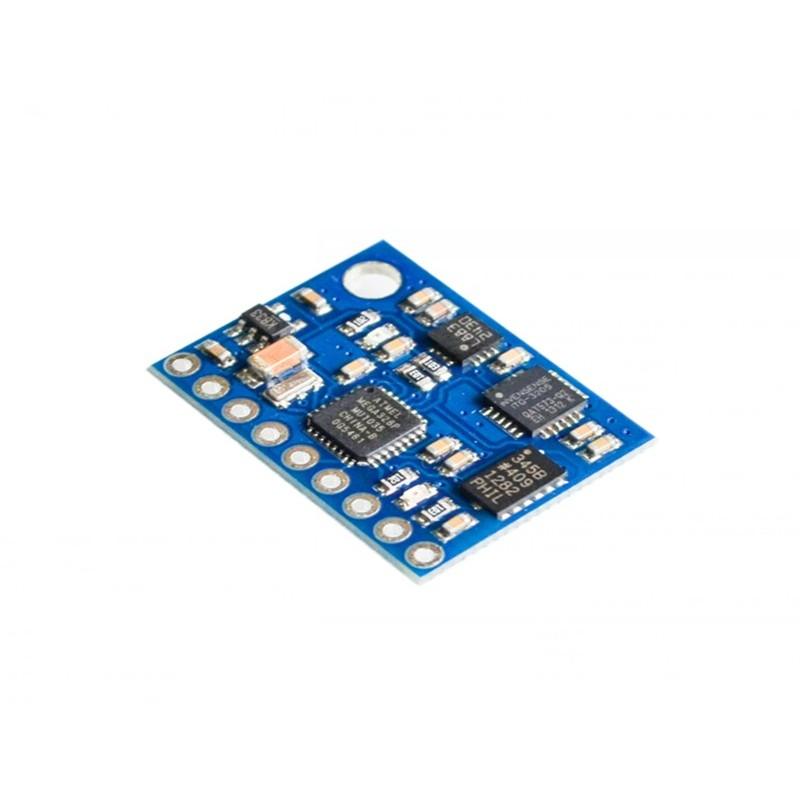
\includegraphics[width=0.55\textwidth]{images/chapter/design/components/final_IMU.png}  % Adjust the width as necessary
    \caption{9DOF GY-85 - ITG3205 + ADXL345 + HMC5883L}
    \label{fig:9DOF GY-85 - ITG3205 + ADXL345 + HMC5883L}        
\end{figure}

\textbf{SIM7000E Arduino NB-IoT/LTE/GPRS/GPS Expansion Shield}
\\\\
The \textbf{SIM7000E Expansion Shield} is a versatile communication module designed for use with Arduino boards. It integrates the \textbf{SIM7000E} cellular module, enabling support for multiple communication technologies, including:

\begin{itemize}
    \item \textbf{NB-IoT (Narrowband IoT)} for low-power, wide-area communication,
    \item \textbf{LTE Cat-M1} for efficient, low-latency data transmission,
    \item \textbf{GPRS/EDGE} as a fallback for 2G networks,
    \item \textbf{GPS} for accurate positioning and navigation.
    \item \textbf{Amperage consume} of 1 mA as it requests for data transferece.
\end{itemize}

The shield is ideal for IoT applications requiring reliable connectivity and 
geolocation, such as asset tracking, environmental monitoring, smart 
agriculture, and remote sensing. It interfaces easily with Arduino via UART, 
making it accessible for both prototyping and deployment in embedded systems.

\begin{figure}[H]
    \centering
    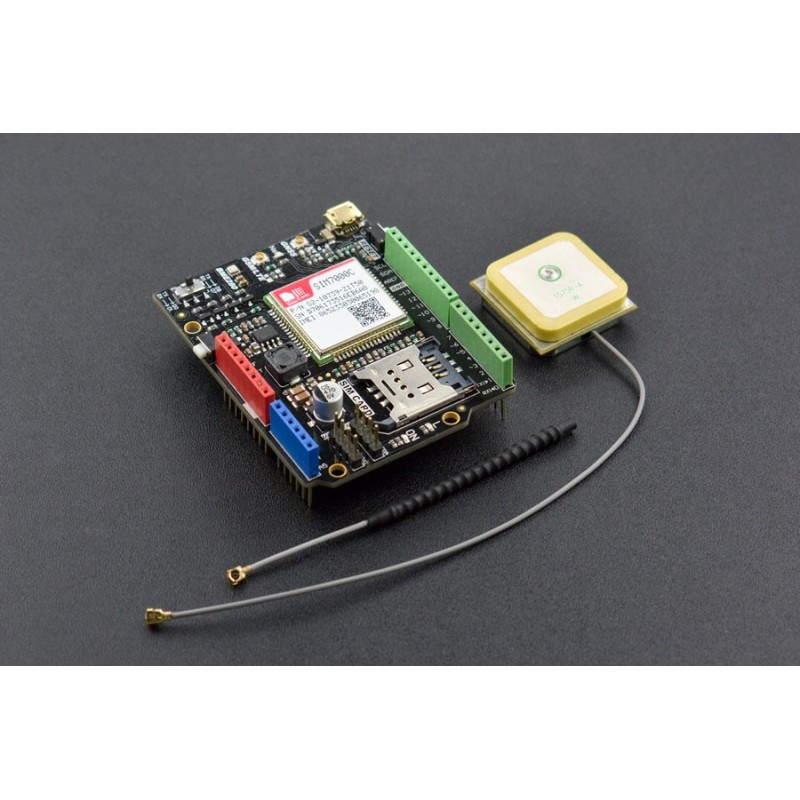
\includegraphics[width=0.7\textwidth]{images/chapter/design/components/SIM7000.png}  % Adjust the width as necessary
    \caption{SIM7000E}
    \label{fig:SIM7000E}        
\end{figure}

\textbf{Waterproof Temperature Sensor (DS18B20)}\\\\
The \textbf{DS18B20} is a digital temperature sensor known for its accuracy, reliability, and ease of use. Encapsulated in a waterproof stainless steel probe, this version of the sensor is ideal for use in wet or outdoor environments.

Key features include:

\begin{itemize}
    \item \textbf{Temperature range}: -55°C to +125°C,
    \item \textbf{Accuracy}: ±0.5°C in the -10°C to +85°C range,
    \item \textbf{Digital output} via the \textbf{1-Wire} protocol, allowing multiple sensors to share a single data line,
    \item \textbf{Waterproof design} for robust operation in harsh environments.
    \item \textbf{Amperage consume} of 1mA per conversion.
\end{itemize} 

The DS18B20 is commonly used in applications such as HVAC systems, weather
stations, industrial temperature monitoring, and smart farming. Its simple 
interface and compatibility with microcontrollers like Arduino and STM32 
make it a popular choice for both hobbyist and professional projects.

\begin{figure}[H]
    \centering
    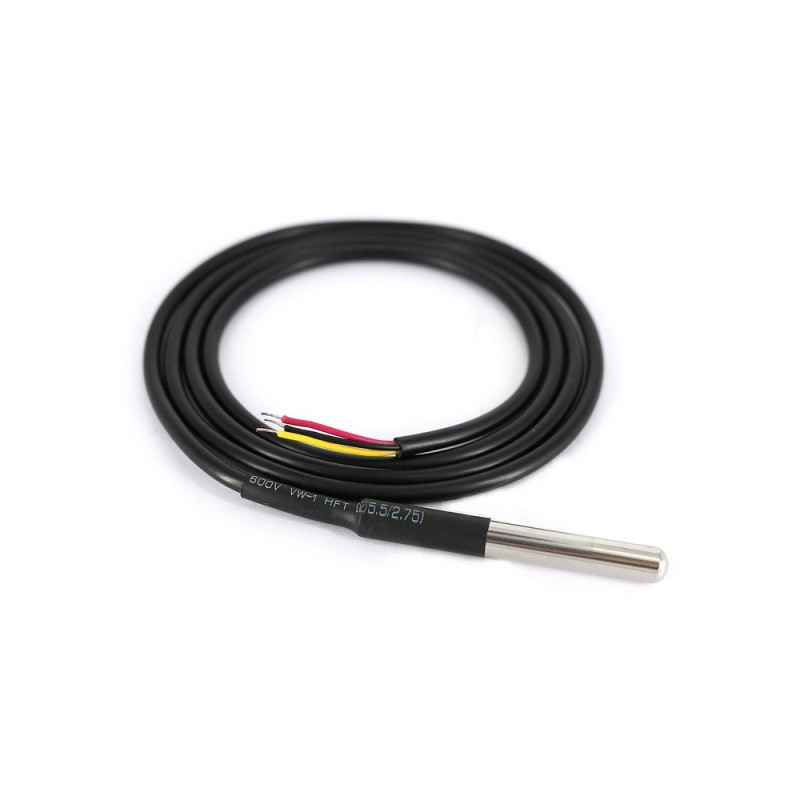
\includegraphics[width=0.70\textwidth]{images/chapter/design/components/temp.png}  % Adjust the width as necessary
    \caption{DS18B20}
    \label{fig:DS18B20}        
\end{figure}
\textbf{Micro SDHC Card INF01016}\\\\
The size  of the SD card, will depend on the amount of data to be stored.
\\\\
\( Storage Size = (Packege Size(bytes) * Time Online(H))/Sample period(H) \)
\\\\
Speculating that 5S will produce around 200 bytes each 10 minutes over 4 months
it is possible to reach the value of 
\\\\
\( Storage Size = (200 * 4 * 30 * 24)/(10/60) = 3.4Gbytes\)
%saize dimention
%sdcard.png

\begin{figure}[H]
    \centering
    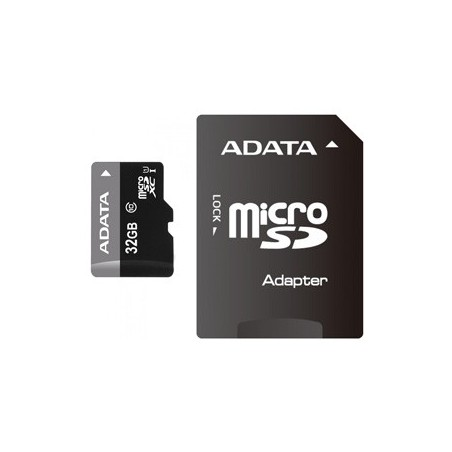
\includegraphics[width=0.6\textwidth]{images/chapter/design/components/sdcard.png}  % Adjust the width as necessary
    \caption{Cartão micro SD}
    \label{fig:Cartão micro SD}        
\end{figure}

\textbf{Micro SDHC Card Reader Module and Battery Holder}\\\\
As the last components, there's will be used some support modules and battery 
support to hold the electronics in place.

\begin{figure}[H]
    \centering
    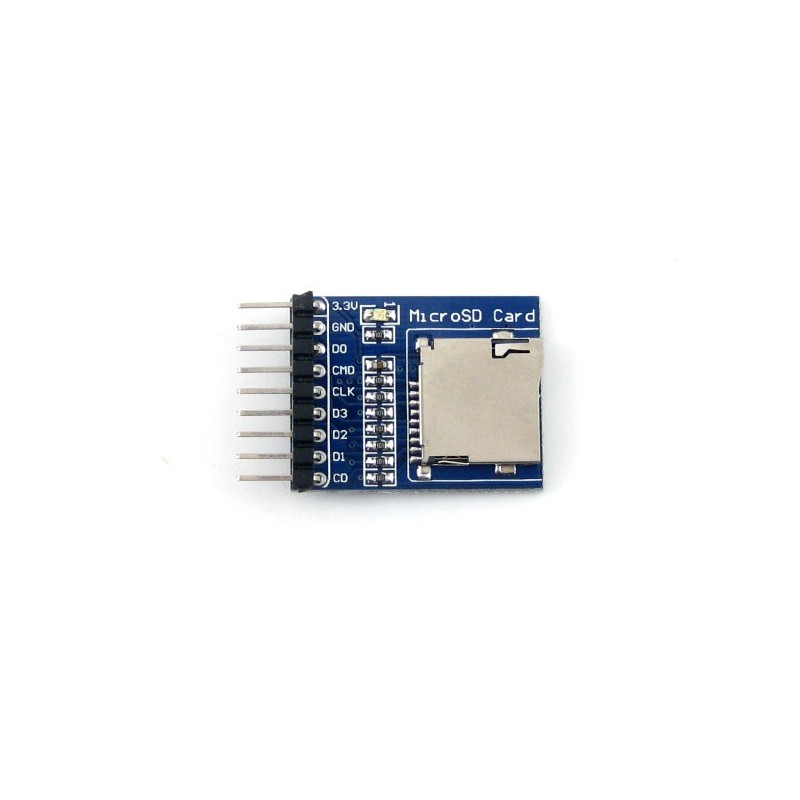
\includegraphics[width=0.3\textwidth]{images/chapter/design/components/sd_support.jpg}  % Adjust the width as necessary
    %\caption{Módulo leitor de cartões micro SD}
    \label{fig:Módulo leitor de cartões micro SD}        
    \hspace{0.1cm}
    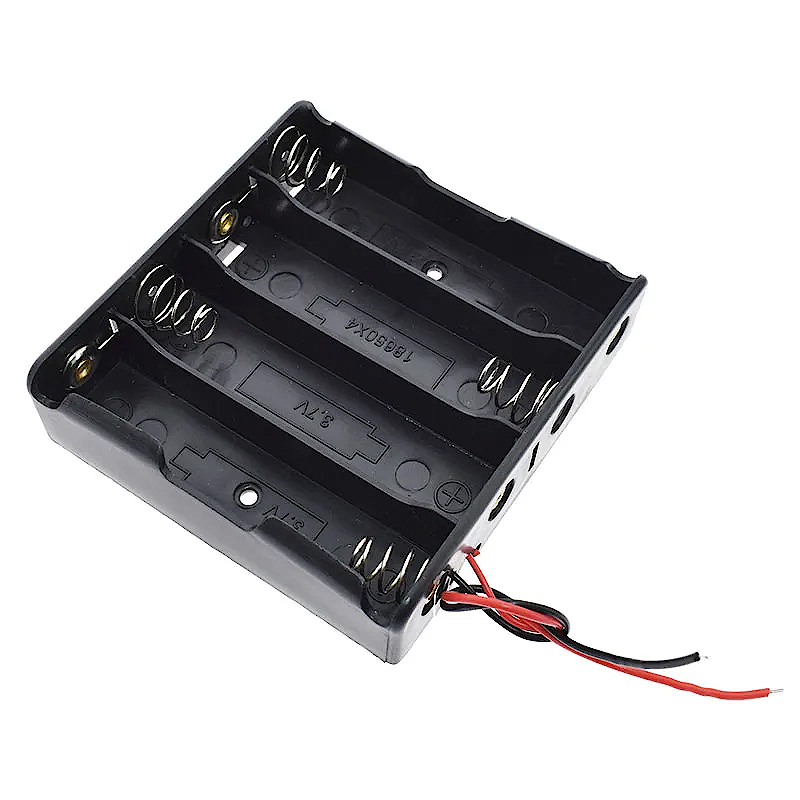
\includegraphics[width=0.2\textwidth]{images/chapter/design/components/battery-holder.jpg}  % Adjust the width as necessary
    \caption{Battery Holder}
    \label{fig:Battery Holder}        
\end{figure}



\subsubsection{Possible Solar Energy}
As an additional topic, here will be briefly explored the option of renewable
energy, for future exploration.

The module AEM10941 and the solar panel SM111K06L are good recommendations.Is ad
visible to follow the datasheet as the module requires specific configuration andcircuits 
to work properly.

%\subsection{SDCard}
%\subsection{STM32}

%STM32L010K4T6
%microcontroler
%ADC
%UART
%SPI
%ONEWire
%\subsection{BMI088 IMU Sensor}
%gyroscope and acelerometer


%\subsection{Temperature}
%DS18B20



\subsubsection{Batteries}

Using the formula \( Battery Capacity = Amperage * Time\), it can be determinate the 
Amperage consumption limit. As Batteries capacity has a discrete value available on market,
it is possible to make a table as graph the results for better visualization.

Using the 3,7V batteries available by the laboratory, the following table can be constructed. 
\\
\begin{table}[h!]
    \centering
    \begin{tabular}{l|l|l}

        Cell Capacity (mAH)& Max Amperage(mA) & price(€) \\
        \hline
        800                & 1,11 & 4,95\\
        2000               & 2,77 & 3,40\\
        2200               & 3,05 & 3,90\\
        2500               & 3,47 & 4,40\\
        2600               & 3,61 & 4,60\\
        3200               & 4.44 & 5,40\\
        3350               & 4.65 & 9,40\\
    \end{tabular}
    \caption{Batteries Capacitis, prices and time relation.}
    \label{table: Batteries Capacitis, prices and time relation.}
\end{table}

However, 1 mouth is a short amount of time when the IPC cycle take almost one third of 
the year. Then, using more batteries, 5S will accomplish to acquire date of a full cycle.
As the equation for the Amperage consumption is linear, multiplying the amount of time by 
four implies four times the capacity meaning the system will 



%batt.jpg

\begin{figure}[H]
    \centering
    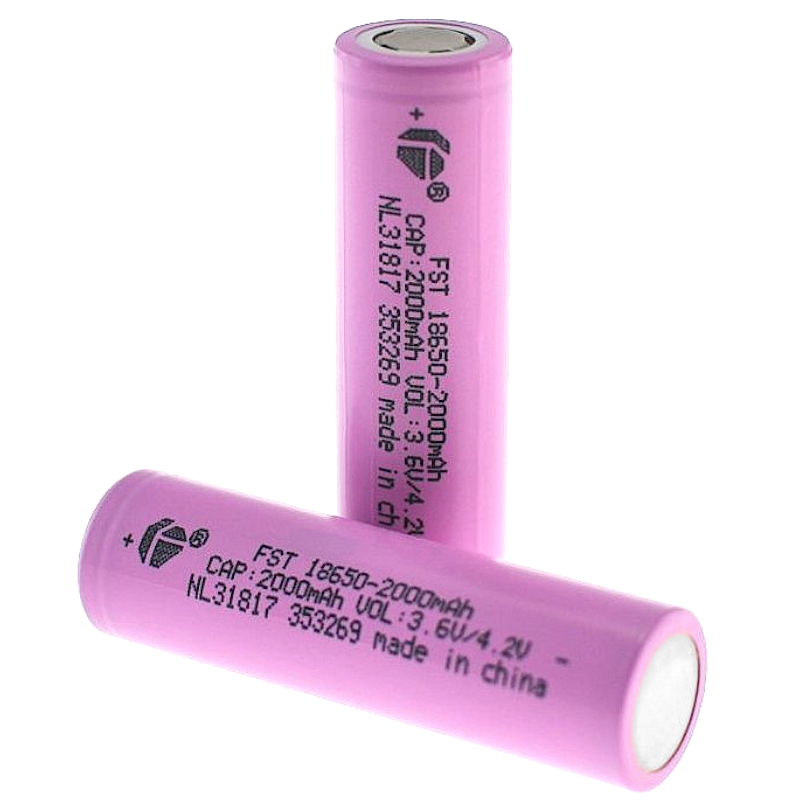
\includegraphics[width=0.6\textwidth]{images/chapter/design/components/batt.jpg}  % Adjust the width as necessary
    \caption{LI-ION 18650 3,7V 2000MAH}
    \label{fig:Battery}        
\end{figure}

\subsection{System Pinout}

Here will be displayed the systems pinout. (Yet to be decided)

\begin{table}[h!]
    \centering
    \begin{tabular}{l|l|l}

        Name & Pinout & uC Pin \\
        \hline
        Temperature Sensor & VDD  & 3.3V\\
                           &      &     \\
        IMU                & VDD  & 3.3V\\
                           &      &     \\
        UART AT            & 3,05 & 3,90\\
                           &      &     \\
        UART DEBUG         & 3,47 & 4,40\\
                           &      &     \\
        ADC                & 3,61 & 4,60\\
                           &      &     \\
        SD card            & VDD  & 3.3V\\
                           &      &     \\
    \end{tabular}
    \caption{Batteries Capacities, prices and time relation.}
    \label{table: Batteries Capacities, prices and time relation.}
\end{table}

\section{Shell}
2.5 dB Antenna should be at least 15 cm form water 


\subsection{Conclusion}

Diagram


The hardware configurations, as indicated on the datasheet should follow the leading steps.
%hw config

As for the UART communication, the list of commands are listed on the datasheet. 
As for better flow, here are listed the commands used along the project and their functionalities. 
%commmand list


\section{Tools and COTS}
\subsection{Tools}
\subsubsection{Inkscape}
A free and open-source vector graphics editor used for creating and editing SVG-based diagrams, schematics, and illustrations. Useful for generating custom graphics, PCB artwork, and documentation visuals.
\subsubsection{draw.io}
A web-based diagramming tool for creating flowcharts, system architectures, block diagrams, and wiring schematics. Supports real-time collaboration and integrates with cloud services like Google Drive and GitHub.
\subsubsection{STM32 CUBEmx}
A configuration and code generation tool for STM32 microcontrollers. Simplifies peripheral setup, clock tree configuration, and generates initialization C code for use with IDEs like STM32CubeIDE or Keil.
\subsubsection{Fusion360}
A professional-grade 3D CAD, CAM, and CAE tool from Autodesk. Used for mechanical design, simulation, and 3D modeling, making it ideal for designing enclosures, mounts, and mechanical parts.
\subsubsection{\LaTeX}
A high-quality typesetting system used for technical and scientific documentation. Ideal for creating well-formatted reports, theses, datasheets, and documentation with complex mathematical content
\subsubsection{Minicom}
Minicom is a text-based serial communication program for Unix-like systems. It allows you to connect to serial devices (like routers, microcontrollers, or modems) via a serial port (e.g., /dev/ttyACM0). It's commonly used for debugging, configuration, and monitoring of hardware over UART.
\subsection{COTS}
All COTS are specified on the \hyperref[link:Board Consumption]{Board Consumption} chapter.
%\section{Theorical Concepts}
    
    \newpage
    \chapter{Implementation}
\section{Hardware}

\section{Software}

use DMA to sample withou using the cpu
\subsection{DataBase Comunication}
Mongo db \\
JASON

    \newpage
    \chapter{Conclusion}
\section{Gantt Diagram}
\section{Bibliografy}
    
\end{document}